Для определения температуры печи используется термопара, позволяющаю находить относительное изменение температуры, однако абсолютное значение $T_0$ было не откалибровано. Для калибровки термопары использо вался следующий метод. Атомарный пучок, выходящий из печи, подсвечивался резонансным лазерным излучением на длине волны $410$ нм, соответсвтвующей переходу $\ket{F=4} \to \ket{F=5}$ \cite{vlad}. Фотодиодом измерялось интегральное значение флюоресценции  $\subt{V}{PD}$ атомов в пучке для различных значений отстройки лазера $\delta$ (рис. \ref{fig:oven}а), примеры приведены на рис. \ref{oven}a. Верно, что в резонансе максимум интенсивности пропорционален потоку атомов $\sub{\Phi}{tot}$. Действительно, нелинейные эффекты связанные с изменением геометрии системы можно связать с изменением наиболее вероятной тепловой скорости $\alpha \propto \sqrt{T}$, но из зависимости \eqref{oven} видно, что $\sub{\Phi}{tot}(T) \propto \sub{n}{sat}(T)$ и, соответственно, экспоненциально зависит от температуры \eqref{nTp}, что и определяет основной характер зависимости. 


\begin{figure}[ht]
    \centering
    \subfigure[]{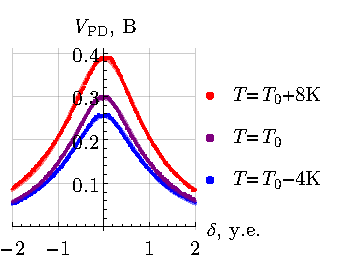
\includegraphics{figs/ovenD_v2.pdf}}
    \hspace{5 mm} 
    \subfigure[]{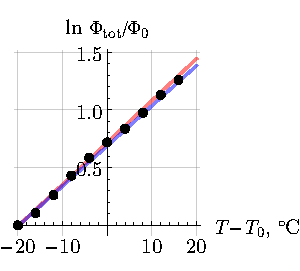
\includegraphics{figs/oven1_v4.pdf}}
    \subfigure[]{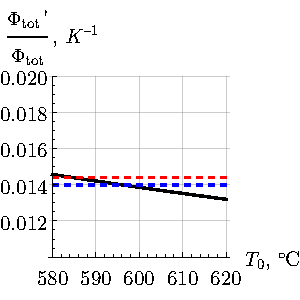
\includegraphics{figs/oven2_v4.pdf}}
    \vspace{-3mm}
    \caption{a) Снятая экспериментальная зависимость мощности флюоресценции атомарного пучка от величины отстройки от резонанса лазерного излучения. Непрерывным линиями показана аппроксимация данных лоренцовым контуром. б) Относительная зависимость потока атомов из печки $\sub{\Phi}{tot}$ от температуры: черными точками отмечены экспериментально снаятые точки, непрерывными линиями отмечены границы линейной апроксимации  в) Восстановление значения $T_0$ по относительному изменению потока: черным обозначена теоретическая зависимость \eqref{nTp}, штрихованным линиями обозначены границы аппроксимации экспериментальных данных уровня}
    \label{fig:oven}
\end{figure}


Итак, найдём логарифмическую производную $\sub{\Phi}{tot}'/\sub{\Phi}{tot}$, с помощью линейной аппроксимации зависимости $\ln \sub{\Phi}{tot} / \sub{\Phi}{0}$ (рис. \ref{fig:oven}б), где $\Phi_0 = \sub{\Phi}{tot}(T=T_0 - 20 \dC)$. Решая уравнение $\sub{n}{sat}'/\sub{n}{sat} = \sub{\Phi}{tot}'/\sub{\Phi}{tot} = \subt{V}{PD}' / \subt{V}{PD}$, находим (рис. \ref{fig:oven}в) 
\begin{equation}
    T_0 = (590 \pm 10) \dC.
\end{equation}
% \red{(полученное значение согласуется с экспериментом по реперной точке на температуре плавления алюминия, стоит ли эту историю описывать?)}.

